\section{Localisation}
\subsection{Method}
For the localisation part of the project it was chosen to compare two different approaches:

\begin{itemize}
	\item Position estimate based on odometry (wheel encoders).
	\item Position estimate based on line features extracted from the laserrange scanner. 
\end{itemize}

Both of these approaches rely on a known starting location. The second also needs knowledge of the environment - it must  compare the extracted features with probable features from the map (based on last know location of the robot). 


The mobile robot used is a "Nexus Robot - 2WD mobile robot kit 10004", fitted with a laserrange scanner of type "Hokuyo URG-04LX-LG". 

\begin{figure}[ht]
\centering
  \begin{subfigure}[t]{0.3\textwidth}
    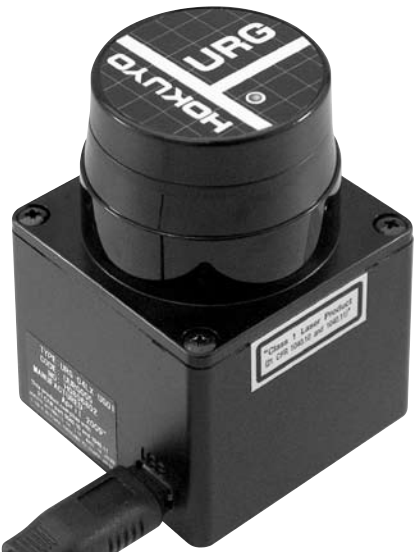
\includegraphics[width = \textwidth]{graphics/hokuyo_laserrange}
    \caption{Hokuyo URG-04LX-LG laserrange scanner.}
    \label{laserrange}
  \end{subfigure}
  \begin{subfigure}[t]{0.4\textwidth}
    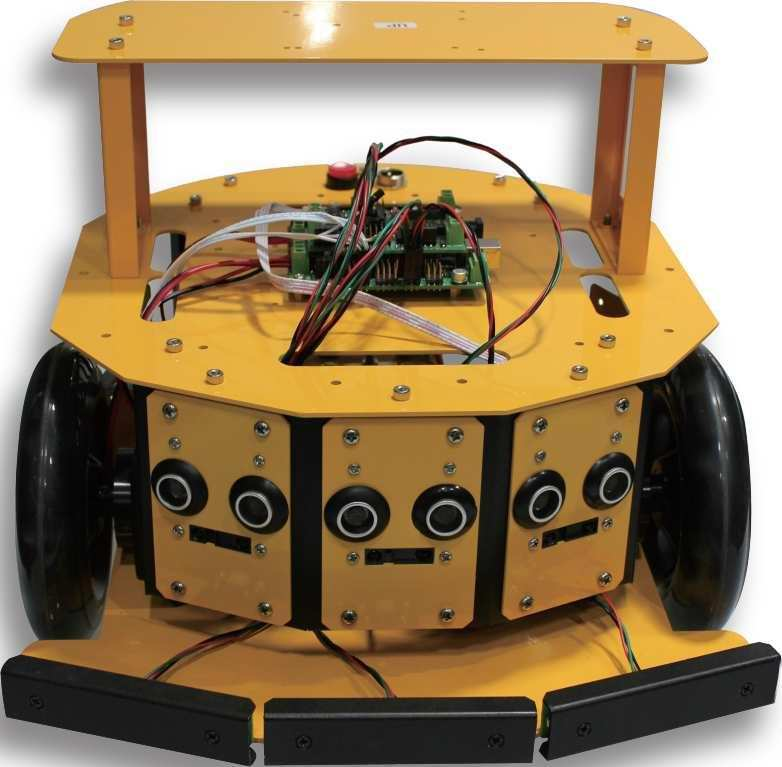
\includegraphics[width = \textwidth]{graphics/nexus_robot}
    \caption{Nexus Robot - 2WD mobile robot kit 10004}
    \label{laserrange}
  \end{subfigure}
\end{figure}


The performance of the localization technique was measured using UMB-mark. 
The position before and after following a preprogrammed path through a 1 x 1 [m] square 10 times was compared. 
While testing, the robot only used sensor feedback from the encoders. 
Sensor readings from both the encoders and the laserrange scanner was gathered, and saved for further offline processing. 

\subsubsection{Position based on odometry}
\todo[inline, author=Michael]{Based on (or ripped off :P ) sec. 5.2.4 from our lovely friend, siegwart.}
The position/state of the robot is represented by the vector: 
\begin{equation}
  p = 
  \begin{bmatrix}
    x \\
    y \\
    \theta 
  \end{bmatrix}
\end{equation}
The robots position is estimated from the previous position + the movement in the last time period $\Delta t$. The change in position $\Delta p$ from each timestep is added to the position. This can be written as 
\begin{equation}
  p\textrm' = p + \Delta p
\end{equation}
The feedback from the robot is given as the movement of each wheel in millimetres. $\Delta p$ can be from the following equations: 
\begin{eqnarray}
	\Delta x &=& \Delta s \cos \left(\theta + \frac{\Delta \theta}{2}\right) \\
	\Delta y &=& \Delta s \sin \left(\theta + \frac{\Delta \theta}{2}\right) \\
	\Delta \theta &=& \frac{\Delta s_r + \Delta s_l}{b} \\
	\Delta s &=& \frac{\Delta s_r + \Delta s_l}{2} \\
\end{eqnarray}
Where $\Delta s_r; \Delta s_l$ = distance traveled by right and left wheel and $b$ is the distance between the robots two wheels. Adding this together, the equation for the updated position is: 
\begin{equation}
  p\textrm' = 
  \begin{bmatrix}
    x \\
    y \\
    \theta 
  \end{bmatrix}
  +
  \begin{bmatrix}
    \Delta s \cos \left(\theta + \frac{\Delta \theta}{2}\right) \\
    \Delta s \sin \left(\theta + \frac{\Delta \theta}{2}\right) \\
    \frac{\Delta s_r + \Delta s_l}{b}
  \end{bmatrix}
\end{equation}
\todo[inline, author=Michael]{Maybe add an interfacing of scanner subsubsection here?}
\input{./content/localisation/ransac}

\subsubsection{Position based on features from laserrange scanner}

\begin{figure}
  \includestandalone{./content/localisation/flowchart}
  \caption{The localisation method}
  \label{fig:localisation}
\end{figure}

